\documentclass{beamer}
\usepackage{tikz}
\usepackage{float}
\usepackage{graphicx}
\usepackage[most]{tcolorbox}
\usepackage{comment}
\usetikzlibrary{decorations.pathreplacing}
\tcbuselibrary{theorems}
\tcbset{enhanced,colframe=blue!20,colback={black!5!white},drop shadow}
\setbeamertemplate{section in toc}[sections numbered]
\setbeamertemplate{subsection in toc}[subsections numbered]
\usetheme[numbering=fraction]{metropolis}           % Use metropolis theme
\title{Bachelor Thesis Marginal-Sampling}
\date{17.09.2020}
\author{Michael Fedders}

\newcommand{\s}{\sigma^2}
\newcommand{\sh}{\hat{\sigma}^2}
\newcommand{\y}{\overline{y}}
\newcommand{\R}{\mathbb{R}}
\newcommand{\dx}{\, \mathrm{d}}
\begin{document}
	\maketitle
  	\begin{frame}[plain]
		\frametitle{Table of Contents}
		\tableofcontents
	\end{frame}
	
	\begin{frame}{Small repetition}
		We are dealing with the case 
		\[
		\overline{y}_{k} = c + (h(x(t_k,\theta)) + \varepsilon_{k}
  		\]
  		where
  		\begin{itemize}
  		\item $\y_k$ is the data
  		\item $c$ is the offset parameter
  		\item $h$ is the observation function
  		\item $\varepsilon_k$ is the noise
  		\end{itemize}
	\end{frame}		
	
	
	
\section{Normal-Gamma Prior}

	\begin{frame}{Environment}
		In contrast to last time we now assume the two priors from our likelihood 			are now a joint probability distribution, the so called normal-gamma 				distribution. \\
		The two parameters which we want to marginalize are the offset parameter $c$ 		and the precision $\lambda$, which is the same as $1/\s$.
	\end{frame}
  	
  	\begin{frame}{prior-definition}
  		The normal-gamma prior depends on 4 shape parameters, $\mu, \kappa, 				\alpha, \beta$ and has the following structure:
  		\begin{align}
  			p(c, \lambda) &= f(c, \lambda \mid \mu, \kappa, \alpha, \beta) \\
  			&= \mathcal{N}(c \mid \mu, 1/(\kappa \lambda)) \cdot \Gamma(\lambda 				\mid \alpha, \beta).
  		\end{align}
  	\end{frame}
  	
  	\begin{frame}{likelihood}
  		As a result the likelihood is
  		\begin{align}
  			 p(D \mid \theta, c, \lambda) = \biggl(\frac{\lambda}{2\pi}\biggr)					^{N/2} \cdot \exp\left( - \frac{\lambda}{2} \sum_{k = 1}^N (\y_k - (c 				+ h_k))^2 \right)
  		\end{align}
  	\end{frame}
  	
	\begin{frame}{Calculation}
  		We can start with the usual setup:
  		\begin{align}
    		p(D \mid \theta) &= \int_{\R \times \R_+} p(D \mid \theta,c,\lambda) 				p(c, \lambda) \, d(c, \lambda)
		\end{align}
  	\end{frame}  	
  	
  	\begin{frame}{Calculation}
  		We can start with the usual setup:
  		\begin{align}
    		p(D \mid \theta) &= \int_{\R \times \R_+} p(D \mid \theta,c,\lambda) 				p(c, \lambda) \, d(c, \lambda) \\
    		&= \int_{\R_+} \int_\R \biggl(\frac{\lambda}{2\pi}\biggr)^{N/2} \exp				\left( - \frac{\lambda}{2} \sum_{k = 1}^N (\y_k - (c + h_k))^2 \right) 			\cdot \\
    		& \frac{\beta^\alpha \sqrt{\kappa}}{\Gamma(\alpha)\sqrt{2\pi}} 						\lambda^{\alpha-1/2} \exp\left(- \frac{\lambda}{2} [\kappa (c - \mu)^2 			+ 2\beta] \right) \, dc \, d\lambda
		\end{align}
  	\end{frame}
  	
  	\begin{frame}{Offset Integration}
  		We pull out the constants and terms which only rely on $\lambda$ to 				integrate over $c$.
  		\begin{align}
   			& \int_\R \exp \left( -\frac{\lambda}{2} \left( \left( \sum_{k = 1}^N 				((\overline{y_k} - h_k)  - c)^2 \right) + \kappa(c - \mu)^2 +2\beta 				\right) \right) \, dc \\
    		&= \int_\R \exp \Biggl( -\frac{\lambda}{2} \Biggl( (N + \kappa) c^2 - 				2 \Biggl(\Biggl(\sum_{k = 1}^N \overline{y_k}-h_k \Biggr) + \kappa \mu 			\Biggr) c \\
    		&+ \Biggl( \sum_{k = 1}^N (\overline{y_k} - h_k)^2 \Biggr) + \kappa 				\mu^2 + 2\beta \Biggr) \Biggr) \, dc
		\end{align}
  	\end{frame}
  	
  	\begin{frame}{Offset Integration}
  		Now we can use the exponential integration formula:
  		\[
  			\int_\R \exp(-a \cdot c^2 + b \cdot c - d) \, dc = \sqrt{\frac{\pi}					{a}} \cdot \exp \biggl( \frac{b^2}{4a} - d \biggr)
  		\]
  	\end{frame}  	
  	
  	\begin{frame}{Offset Integration}
  		Now we can use the exponential integration formula:
  		\[
  			\int_\R \exp(-a \cdot c^2 + b \cdot c - d) \, dc = \sqrt{\frac{\pi}					{a}} \cdot \exp \biggl( \frac{b^2}{4a} - d \biggr)
  		\]
  		and receive
  		\begin{align}
  			& \sqrt{\frac{2 \pi}{\lambda(N + \kappa)}} \cdot \exp \Biggl( \lambda 				\cdot \Biggl( \frac{1}{2(N + \kappa)} \Biggl(\Biggl(\sum_{k = 1}^N 					\overline{y_k} - h_k\Biggr)+ \kappa \mu \Biggr)^2 \\
    		&- \frac{1}{2}\Biggl( \Biggl( \sum_{k = 1}^N (\overline{y_k} - h_k)^2 				\Biggr) + \kappa \mu^2 + 2\beta \Biggr) \Biggr) \Biggr)
  		\end{align}
  	\end{frame}
  	
  	\begin{frame}{Offset Integration}
  		In total we have the integral
  			\[
  				\frac{\beta^\alpha}{\Gamma(\alpha) (2\pi)^{\frac{N}{2}}} \cdot 						\sqrt{\frac{\kappa}{N + \kappa}} \int_{\R_+} \lambda^{\alpha + 						\frac{N}{2} - 1} \cdot e^{-\lambda \cdot C} \, d\lambda,
  			\]
  		while $C$ is a constant.
  	\end{frame}
  	
  	\begin{frame}{Final steps}
  		Together with the substitution of $\varphi (\lambda) = C \cdot \lambda$ 			and the knowledge about the gamma-function we conclude with the following 			form:
  		\[
  			\frac{(\beta / C)^\alpha}{\Gamma(\alpha) (2\pi C)^{\frac{N}{2}}} \cdot 			\sqrt{\frac{\kappa}{N + \kappa}} \cdot \Gamma \biggl(\frac{N}{2} + 					\alpha \biggr)
  		\]
   	\end{frame}
   	
   	\begin{frame}{Numerical Testing}
   		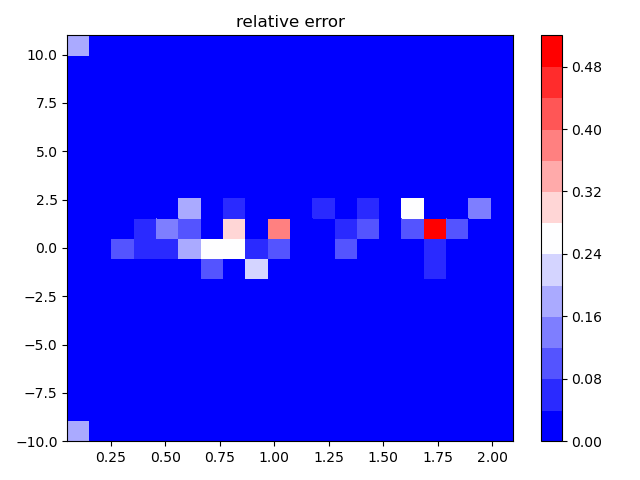
\includegraphics[scale=0.45]{relative_error.png}
   	\end{frame}
\begin{comment}   	
\section{Log-Normal noise}

	\begin{frame}{Log-Normal likelihood}
		We make the assumption that $\varepsilon_k \sim e^{\sigma \cdot Z}$, i.e. 			it has a  log-normal distribution. The new likelihood has the following 			form:
		\begin{align}
			p(D \mid \theta, c, \sigma^2) &= \prod_{k = 1}^N \frac{1}{\y_k - c 					- h_k}\mathcal{N}\bigl( \ln\bigl(\y_k - c - h_k\bigr) \mid 0, \s\bigr) 			\\
			&= \prod_{k = 1}^N \frac{1}{\sqrt{2\pi\s}} \cdot \exp\biggl(-\frac{1}				{2\s}\bigl(\ln^2(y_k - c - h_k) \\
			& + 2\s \cdot \ln(y_k - c - h_k)\bigr)\biggr)
		\end{align}
	\end{frame}

	\begin{frame}{Integration}
		Problem: We can't substitute here as every $\ln(\y_k - c - h_k)$ part has 			a different substraction and the logarithm can't be summed up.
		We can still try to marginalize out sigma but there comes another problem 			into hand which I will show at the next example.
	\end{frame}
\end{comment}

\section{Laplacian noise}

	\begin{frame}{Laplacian likelihood}
		We make the assumption that $\epsilon_k \sim Laplace(0, \sigma), \sigma 			\in (0, \infty)$, i.e. it has a  Laplace distribution. The new likelihood 			has the following form:
		\begin{align}
    		p(D \mid \theta, c, \sigma) &= \prod_{k = 1}^N Laplace(\y_k\mid c + 				h_k, \sigma) \\
    		&= \prod_{k = 1}^N \frac{1}{2\sigma} \cdot \exp \left\{- 							\frac{\lvert \y_k - c- h_k \lvert}{\sigma} \right\}
		\end{align}
	\end{frame}
	
	\begin{frame}{Marginalisation Integral}
		The integral we receive is

		\begin{align}
    		&\iint p(D \mid \theta, c, \sigma) p(c) p(\sigma) \dx c \dx \sigma \\
    		&= \int_0^{\infty} \int_{-\infty}^{\infty} \prod_{k = 1}^N \frac{1}					{2\sigma} \cdot \exp \left\{- \frac{\lvert c - (\y_k -h_k) \lvert}					{\sigma} \right\} p(c) p(\sigma) \dx c \dx \sigma
		\end{align}
	\end{frame}
	
	\begin{frame}{Calculation}
		For calculation-reasons we renumber $\y_k$ and $h_k$ so that $y_k - h_k$ 			are ordered from smallest to biggest, i.e. $\y_1 - h_1$ is the smallest 			number, $\y_N - h_N$ the biggest.
		Then we choose $b_0 = -\infty, b_i = \y- h_i (i = 1, \ldots, N), b_{N+1} = 		\infty$. Now we can split up the integral in the following parts:
		\begin{align}
    		\int_0^{\infty} \sum_{i = 0}^N \int_{b_i}^{b_{i+1}} \frac{1}{2\sigma} 				\exp \left\{- \frac{\sum_{k = 1}^N \lvert c - (\y_k - h_k)\lvert} 					{\sigma} \right\} p(c) p(\sigma) \dx c \dx \sigma
		\end{align}
	\end{frame}
	
	\begin{frame}{Calculation}
		To remove the absolute value, we introduce the index $R_{k, i}$ which is 			defined like this:
		\[
			r_{k, i} =
			\begin{cases}
    			1 & \text{if} \, k \leq i \\
    			-1 & \text{else}
			\end{cases}
		\]
	\end{frame}
	
	\begin{frame}{Calculation}
		\begin{align}
    		&\int_0^{\infty} \frac{1}{2\sigma} \sum_{i = 0}^N p(\sigma) \int_{b_i}				^{b_{i+1}} \exp \underbrace{\left\{-\frac{\sum_{k = 1}^N r_{k, i} (c - 			(\y_k - h_k))}{\sigma} \right\}}_{= (*)} \dx c \dx\sigma \\
    		&\text{with} \, (*) = \frac{-c (i - (N -i)) + \sum_{k = 1}^i \y_k - 				h_k - \sum_{i + 1}^N \y_k - h_K}{\sigma} \\
    		&= \int_0^\infty \frac{1}{2\sigma} p(\sigma) \sum_{i = 0}^N \exp \left				\{\frac{\sum_{k = 1}^i \y_k - h_k - \sum_{i + 1}^N \y_k - h_K}{\sigma}				\right\} \\ \
    		&\cdot \int_{b_i}^{b_{i + 1}} e^{-c(2i -N)} \dx c \dx \sigma
		\end{align}
	\end{frame}
	
	\begin{frame}
		\begin{align}
    & \int_0^\infty \frac{1}{2\sigma} \sum_{i = 1}^{N - 1} \exp \left\{\frac{\sum_{k = 1}^i \y_k - h_k - \sum_{i + 1}^N \y_k - h_K}{\sigma}\right\} \frac{1}{N - 2i} \\
    & \cdot \Bigl(e^{-b_{i + 1}(2i - N)} - e^{-b_i(2i - N)} \Bigr) \dx \sigma  \\
    & + \int_0^\infty \frac{1}{2\sigma} \exp\left\{\frac{-\sum_{k = 1}^N \y_k - h_k}{\sigma} \right\} \underbrace{\int_{-\infty}^{b_1} e^{Nc} \dx c}_{\frac{1}{N}e^{N b_1}} \dx \sigma \\
    &+ \int_0^\infty \frac{1}{2\sigma} \exp\left\{\frac{\sum_{k = 1}^N \y_k - h_k}{\sigma} \right\} \underbrace{\int_{b_N}^{\infty} e^{-Nc} \dx c}_{\frac{1}{N}e^{-N b_N}} \dx \sigma
\end{align}
	\end{frame}
	
\end{document}





















